\documentclass[english]{SPFShortReport}
\usepackage{subfigure}
\usepackage{spfFigures}
\usepackage{longtable}
\usepackage{url}
\usepackage{gensymb}
\usepackage[yyyymmdd,hhmmss]{datetime}
\reportName{Python calculation for heat pump HP25L-M-WEB}
\reportSubName{Parametric Heat Pump calculation} 
\reportDate{\today \hspace{0.1cm} at: \currenttime \hspace{0.1cm} h} 
\author{Dani Carbonell}
\address{dani.carbonell@solarenergy.ch}
\begin{document}
\begin{table}[!ht]
\begin{small}
\caption{Fitted coefficients for the heat pump.}
\begin{center}
\resizebox{12cm}{!} 
{
\begin{tabular}{l | c c } 
\hline
\hline
Coefficient &Description & \\ 
 & &$[kW]$\\ 
\hline
$PQ_{1}$ & \emph{$1^{st}$ condenser polynomial coefficient}  & 2.5033e+01    \\ 
$PQ_{2}$ & \emph{$2^{st}$ condenser polynomial coefficient}  & 2.2522e+02    \\ 
$PQ_{3}$ & \emph{$3^{st}$ condenser polynomial coefficient}  & 7.3843e+01    \\ 
$PQ_{4}$ & \emph{$4^{st}$ condenser polynomial coefficient}  & -8.4936e+01    \\ 
$PQ_{5}$ & \emph{$5^{st}$ condenser polynomial coefficient}  & 3.1917e+02    \\ 
$PQ_{6}$ & \emph{$6^{st}$ condenser polynomial coefficient}  & -4.6866e+02    \\ 
\hline
$PCOP_{1}$ & \emph{$1^{st}$ COP polynomial coefficient}  & 9.6808e+00    \\ 
$PCOP_{2}$ & \emph{$2^{st}$ COP polynomial coefficient}  & 5.3607e+01    \\ 
$PCOP_{3}$ & \emph{$3^{st}$ COP polynomial coefficient}  & -5.5041e+01    \\ 
$PCOP_{4}$ & \emph{$4^{st}$ COP polynomial coefficient}  & -1.7681e+02    \\ 
$PCOP_{5}$ & \emph{$5^{st}$ COP polynomial coefficient}  & 7.0311e+01    \\ 
$PCOP_{6}$ & \emph{$6^{st}$ COP polynomial coefficient}  & 9.0167e+01    \\ 
\hline
$\dot m_{cond}$ & 4500.00 $[kg/h]$\\ 
$\dot m_{evap}$ & 11250.00 $[kg/h]$\\ 
\hline
$COP_{nom}$ (B0W35)& 4.10 \\ 
$Q_{c,nom}$ (B0W35)& 25.20 kW\\ 
$COP_{nom}$ (B2W35)& 4.33 \\ 
$Q_{c,nom}$ (B2W35)& 26.63 kW\\ 
$COP_{nom}$ (B10W35)& 5.31 \\ 
$Q_{c,nom}$ (B10W35)& 32.56 kW\\ 
\hline
\hline
\end{tabular}
}
\label{CoefTable}
\end{center}
\end{small}
\end{table}
\begin{table}[!ht]
\begin{small}
\caption{Predicting results of the heat pump.}
\begin{center}
\resizebox{12cm}{!} 
{
\begin{tabular}{l | c c c c c c c c c c c } 
\hline
\hline
$T_{evap,in}$ &$T_{evap,out}$ &$T_{cond,in}$ &$T_{cond,out}$ &$COP$ &$Q_{cond}$ &$Q_{evap}$ &$W_{comp}$ &$\dot m_{cond}$ &$\dot m_{evap}$ &$\Delta T_{evap}$ &$\Delta T_{cond}$ \\ 
$^oC$ &$^oC$ &$^oC$ &$^oC$ &$[-]$ &$[kW]$ &$[kW]$ &$[kW]$ &kg/h &kg/h &K &K\\ 
\hline
-7.00 & -11.12 & 26.02 & 30.00 & 3.89 & 20.85 & 15.48 & 5.37 & 4500 & 11250 & 4.1 & 4.0\\ 
-7.00 & -10.54 & 34.94 & 38.75 & 3.01 & 19.93 & 13.32 & 6.61 & 4500 & 11250 & 3.5 & 3.8\\ 
-7.00 & -9.74 & 44.05 & 47.50 & 2.32 & 18.08 & 10.29 & 7.79 & 4500 & 11250 & 2.7 & 3.5\\ 
-7.00 & -8.80 & 53.34 & 56.25 & 1.80 & 15.23 & 6.78 & 8.45 & 4500 & 11250 & 1.8 & 2.9\\ 
-7.00 & -7.94 & 62.85 & 65.00 & 1.46 & 11.27 & 3.53 & 7.74 & 4500 & 11250 & 0.9 & 2.2\\ 
-4.00 & -8.64 & 25.64 & 30.00 & 4.22 & 22.85 & 17.44 & 5.41 & 4500 & 11250 & 4.6 & 4.4\\ 
-4.00 & -8.06 & 34.56 & 38.75 & 3.29 & 21.94 & 15.28 & 6.66 & 4500 & 11250 & 4.1 & 4.2\\ 
-4.00 & -7.24 & 43.66 & 47.50 & 2.54 & 20.10 & 12.19 & 7.91 & 4500 & 11250 & 3.2 & 3.8\\ 
-4.00 & -6.25 & 52.95 & 56.25 & 1.96 & 17.27 & 8.47 & 8.80 & 4500 & 11250 & 2.3 & 3.3\\ 
-4.00 & -5.27 & 62.45 & 65.00 & 1.56 & 13.36 & 4.78 & 8.58 & 4500 & 11250 & 1.3 & 2.6\\ 
-1.00 & -6.18 & 25.24 & 30.00 & 4.58 & 24.92 & 19.48 & 5.44 & 4500 & 11250 & 5.2 & 4.8\\ 
-1.00 & -5.60 & 34.17 & 38.75 & 3.59 & 24.00 & 17.31 & 6.69 & 4500 & 11250 & 4.6 & 4.6\\ 
-1.00 & -4.77 & 43.27 & 47.50 & 2.78 & 22.17 & 14.19 & 7.98 & 4500 & 11250 & 3.8 & 4.2\\ 
-1.00 & -3.74 & 52.55 & 56.25 & 2.14 & 19.37 & 10.32 & 9.05 & 4500 & 11250 & 2.7 & 3.7\\ 
-1.00 & -2.66 & 62.04 & 65.00 & 1.68 & 15.50 & 6.25 & 9.24 & 4500 & 11250 & 1.7 & 3.0\\ 
2.00 & -3.73 & 24.84 & 30.00 & 4.95 & 27.04 & 21.58 & 5.46 & 4500 & 11250 & 5.7 & 5.2\\ 
2.00 & -3.16 & 33.76 & 38.75 & 3.90 & 26.12 & 19.43 & 6.70 & 4500 & 11250 & 5.2 & 5.0\\ 
2.00 & -2.33 & 42.86 & 47.50 & 3.03 & 24.30 & 16.28 & 8.02 & 4500 & 11250 & 4.3 & 4.6\\ 
2.00 & -1.27 & 52.14 & 56.25 & 2.33 & 21.51 & 12.30 & 9.22 & 4500 & 11250 & 3.3 & 4.1\\ 
2.00 & -0.11 & 61.62 & 65.00 & 1.81 & 17.69 & 7.93 & 9.76 & 4500 & 11250 & 2.1 & 3.4\\ 
5.00 & -1.31 & 24.42 & 30.00 & 5.34 & 29.22 & 23.74 & 5.47 & 4500 & 11250 & 6.3 & 5.6\\ 
5.00 & -0.74 & 33.35 & 38.75 & 4.23 & 28.30 & 21.61 & 6.70 & 4500 & 11250 & 5.7 & 5.4\\ 
5.00 & 0.10 & 42.44 & 47.50 & 3.30 & 26.49 & 18.45 & 8.03 & 4500 & 11250 & 4.9 & 5.1\\ 
5.00 & 1.17 & 51.72 & 56.25 & 2.54 & 23.72 & 14.40 & 9.32 & 4500 & 11250 & 3.8 & 4.5\\ 
5.00 & 2.40 & 61.20 & 65.00 & 1.96 & 19.93 & 9.78 & 10.15 & 4500 & 11250 & 2.6 & 3.8\\ 
8.00 & 1.10 & 23.99 & 30.00 & 5.74 & 31.45 & 25.98 & 5.48 & 4500 & 11250 & 6.9 & 6.0\\ 
8.00 & 1.66 & 32.92 & 38.75 & 4.57 & 30.54 & 23.86 & 6.68 & 4500 & 11250 & 6.3 & 5.8\\ 
8.00 & 2.50 & 42.01 & 47.50 & 3.58 & 28.73 & 20.71 & 8.02 & 4500 & 11250 & 5.5 & 5.5\\ 
8.00 & 3.59 & 51.29 & 56.25 & 2.77 & 25.98 & 16.60 & 9.38 & 4500 & 11250 & 4.4 & 5.0\\ 
8.00 & 4.87 & 60.76 & 65.00 & 2.13 & 22.22 & 11.79 & 10.42 & 4500 & 11250 & 3.1 & 4.2\\ 
11.00 & 3.49 & 23.56 & 30.00 & 6.16 & 33.74 & 28.27 & 5.48 & 4500 & 11250 & 7.5 & 6.4\\ 
11.00 & 4.04 & 32.48 & 38.75 & 4.93 & 32.83 & 26.18 & 6.66 & 4500 & 11250 & 7.0 & 6.3\\ 
11.00 & 4.88 & 41.58 & 47.50 & 3.88 & 31.03 & 23.04 & 7.99 & 4500 & 11250 & 6.1 & 5.9\\ 
11.00 & 5.98 & 50.85 & 56.25 & 3.01 & 28.29 & 18.90 & 9.39 & 4500 & 11250 & 5.0 & 5.4\\ 
11.00 & 7.29 & 60.31 & 65.00 & 2.32 & 24.56 & 13.95 & 10.61 & 4500 & 11250 & 3.7 & 4.7\\ 
14.00 & 5.86 & 23.11 & 30.00 & 6.60 & 36.09 & 30.62 & 5.47 & 4500 & 11250 & 8.1 & 6.9\\ 
14.00 & 6.41 & 32.03 & 38.75 & 5.31 & 35.18 & 28.55 & 6.63 & 4500 & 11250 & 7.6 & 6.7\\ 
14.00 & 7.24 & 41.13 & 47.50 & 4.20 & 33.38 & 25.43 & 7.95 & 4500 & 11250 & 6.8 & 6.4\\ 
14.00 & 8.34 & 50.40 & 56.25 & 3.27 & 30.66 & 21.28 & 9.37 & 4500 & 11250 & 5.7 & 5.9\\ 
14.00 & 9.68 & 59.85 & 65.00 & 2.52 & 26.95 & 16.24 & 10.72 & 4500 & 11250 & 4.3 & 5.1\\ 
17.00 & 8.22 & 22.65 & 30.00 & 7.05 & 38.50 & 33.04 & 5.46 & 4500 & 11250 & 8.8 & 7.4\\ 
17.00 & 8.76 & 31.57 & 38.75 & 5.70 & 37.59 & 30.99 & 6.59 & 4500 & 11250 & 8.2 & 7.2\\ 
17.00 & 9.59 & 40.67 & 47.50 & 4.53 & 35.79 & 27.90 & 7.90 & 4500 & 11250 & 7.4 & 6.8\\ 
17.00 & 10.69 & 49.93 & 56.25 & 3.54 & 33.08 & 23.75 & 9.33 & 4500 & 11250 & 6.3 & 6.3\\ 
17.00 & 12.05 & 59.39 & 65.00 & 2.73 & 29.40 & 18.64 & 10.76 & 4500 & 11250 & 5.0 & 5.6\\ 
20.00 & 10.56 & 22.18 & 30.00 & 7.52 & 40.96 & 35.51 & 5.45 & 4500 & 11250 & 9.4 & 7.8\\ 
20.00 & 11.10 & 31.10 & 38.75 & 6.11 & 40.05 & 33.49 & 6.56 & 4500 & 11250 & 8.9 & 7.6\\ 
20.00 & 11.91 & 40.19 & 47.50 & 4.88 & 38.26 & 30.42 & 7.84 & 4500 & 11250 & 8.1 & 7.3\\ 
20.00 & 13.01 & 49.46 & 56.25 & 3.84 & 35.56 & 26.29 & 9.27 & 4500 & 11250 & 7.0 & 6.8\\ 
20.00 & 14.38 & 58.91 & 65.00 & 2.96 & 31.90 & 21.14 & 10.76 & 4500 & 11250 & 5.6 & 6.1\\ 
\hline
\hline
\end{tabular}
}
\label{ResultsTable}
\end{center}
\end{small}
\end{table}
\begin{figure}[!ht]
\begin{center}
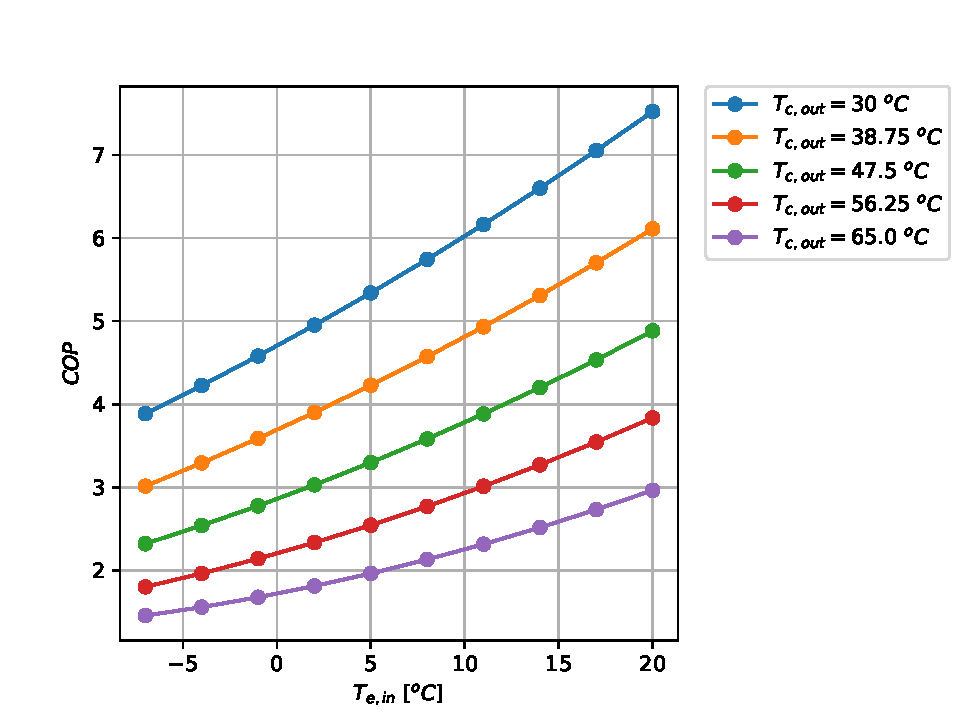
\includegraphics[width=1\textwidth]{C:/Daten/spfPackages/GIT/spfTrnsysFiles/HeatPump/AirToWater/Heliotherm/HP25L-M-WEB/HP25L-M-WEB-Cop.pdf}
\caption{COP Results for the heat pump at the selected points}
\label{COPFig}
\end{center}
\end{figure}
\begin{figure}[!ht]
\begin{center}
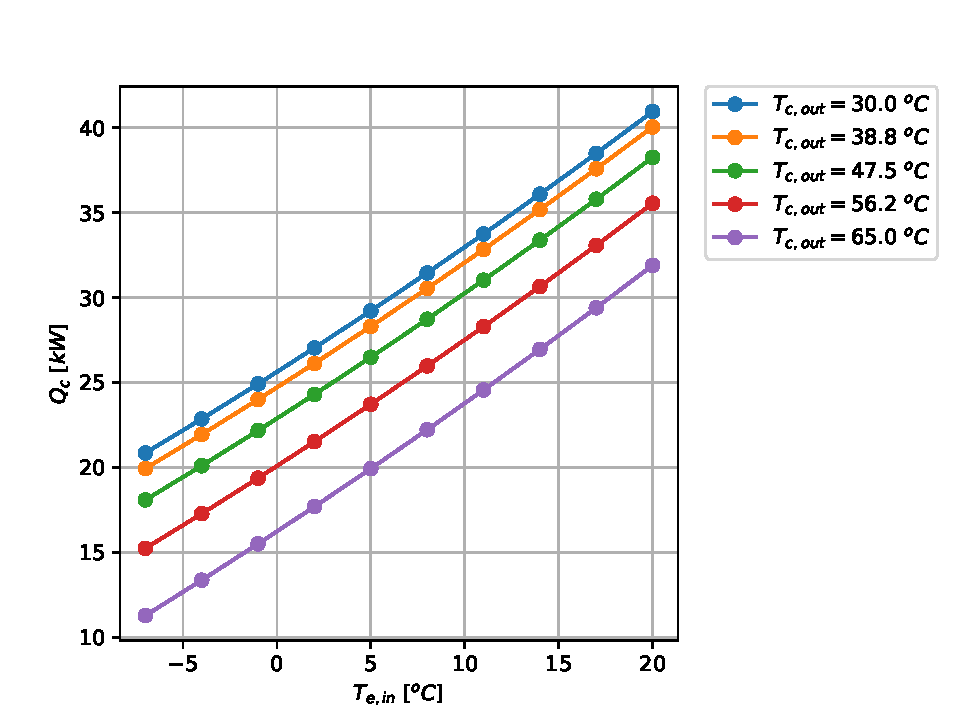
\includegraphics[width=1\textwidth]{C:/Daten/spfPackages/GIT/spfTrnsysFiles/HeatPump/AirToWater/Heliotherm/HP25L-M-WEB/HP25L-M-WEB-Qc.pdf}
\caption{$Q_c$ Results for the heat pump at the selected points}
\label{QcFig}
\end{center}
\end{figure}
\end{document}
